\documentclass[11pt]{article}

\usepackage[utf8]{inputenc}
\usepackage[portuguese]{babel}
\usepackage{indentfirst}
\usepackage{natbib}
\usepackage{graphicx}
\usepackage{float}

\renewcommand{\contentsname}{Índice}

\begin{document}

\begin{titlepage}
   \begin{center}
       
       
\includegraphics[width=0.3\textwidth]{images/EscolaEngenhariaUM.jpeg}
       
       \vspace*{0.5cm}
       
       \textbf{\Large Sistema de gestão de stocks de um	armazém de uma fábrica - Fase 3}

       \vspace{1.3cm}
       \textbf{\large Desenvolvimento de Sistemas de Software}
            
       \vspace{1.3cm}

       Bruno Filipe de Sousa Dias A89583\\ Guilherme Santiago Lopes Pereira A89479 \\ Luís Enes Sousa A89597\\ Pedro Miguel de Soveral Pacheco Barbosa A89529

       \vspace{1.5cm}
       
       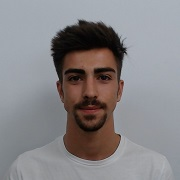
\includegraphics[width=35mm]{images/bruno.jpeg}\hspace{0.2cm}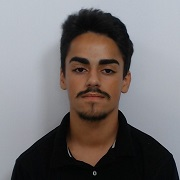
\includegraphics[width=35mm]{images/guilherme.jpeg}
       \vspace{0.15cm}
       \hspace{0.1cm}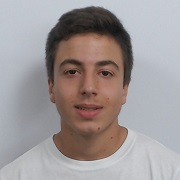
\includegraphics[width=35mm]{images/luis.jpeg}\hspace{0.1cm}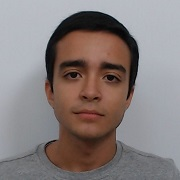
\includegraphics[width=35mm]{images/pedro.jpeg}
       
        
        23 de dezembro de 2020
            
   \end{center}
\end{titlepage}

\tableofcontents
\thispagestyle{empty}
\cleardoublepage

\setcounter{page}{1}

\section{Introdução}

Neste semestre, no âmbito da unidade curricular de Desenvolvimento de Sistemas de Software, foi-nos proposto o desenvolvimento de uma componente de um sistema de gestão de stocks de um armazém de uma fábrica de modo a pôr em prática toda a aprendizagem sobre Desenvolvimento de Sistemos de Software, com auxílio da linguagem de programação orientada aos objetos Java. O seu principal objetivo será desenvolver uma aplicação que suporte alguns cenários descritos no enunciado pelos docentes da cadeira e outros que serão definidos pelo nosso grupo consoante achemos pertinente ao longo da realização deste projeto.

O trabalho foi dividido em três fases de entrega sendo que a terceira consiste na implementação da solução. Para esta finalidade, procedemos ao desenvolvimento dos modelos arquiteturais e comportamentais, especificados a nível de implementação, necessários para os Use Cases especificados pela equipa docente e também à implementação dos mesmos. 

Desta maneira e de forma a conseguirmos implementar a solução final começamos por criar as classes necessárias bem como os seus atributos e métodos. Para isto, recorremos aos diagramas de sequência que elaboramos na 2ª fase deste projeto. Assim, e ao longo da realização desta última fase do projeto, encontramos alguns erros cometidos na fase anterior que precisamos de resolver.

\clearpage

\section{Alterações à Segunda Fase do Projeto}

Ao longo da realização da 3ª fase do projeto apercebemo-nos de que iriamos necessitar de outras classes e que teríamos de mudar alguns métodos e atributos que tinhamos no nosso Diagrama de Classes. Deste modo, elaboramos um Diagrama novo que se encontra na figura seguinte:

\begin{figure}[htb]
    \centering
    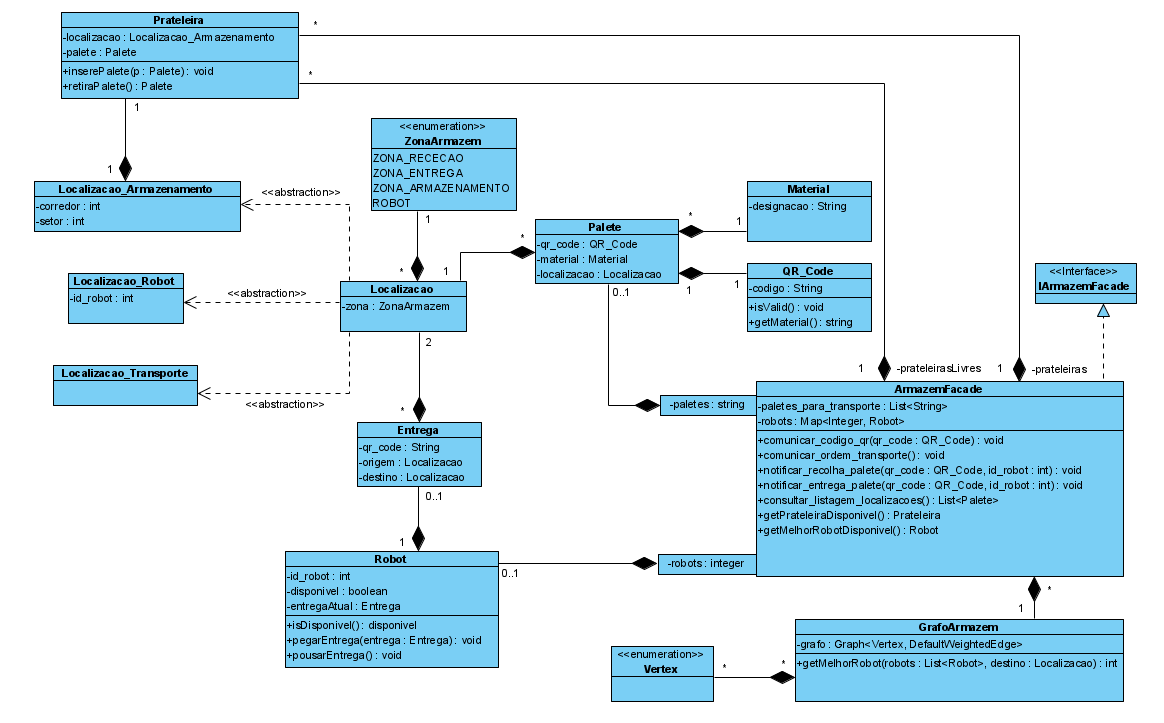
\includegraphics[width=1\textwidth]{images/class_diagram_armazem.png}
    \caption{Diagrama de Classes}
    \label{fig:my_label3}
\end{figure}

\clearpage

\section{Diagrama de ORM}

O Diagrama de ORM é uma evolução do nosso diagrama de classes sendo que inclui as classes DAO's, de modo a implementarmos a persistência.

\begin{figure}[htb]
    \centering
    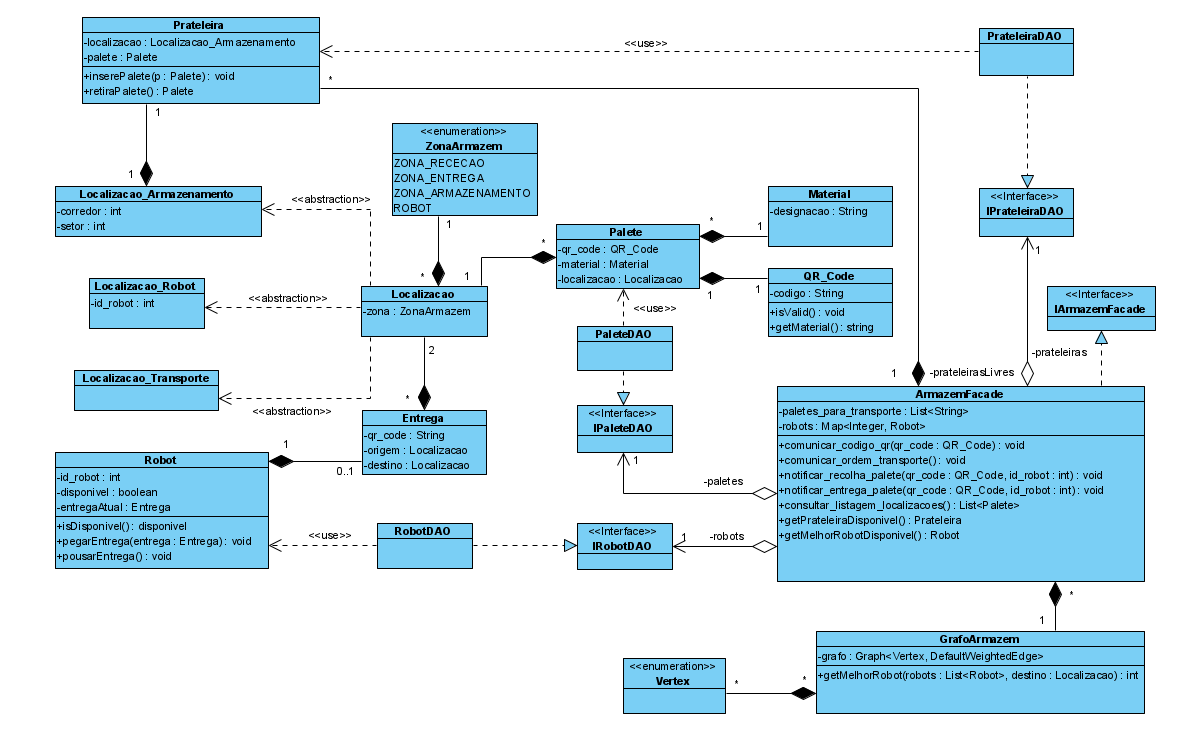
\includegraphics[width=1\textwidth]{images/orm_diagram_armazem.png}
    \caption{Diagrama de ORM}
    \label{fig:my_label3}
\end{figure}

\clearpage

\section{Modelo Lógico da Base de Dados}

Para a criação da nossa Base de Dados procedemos à elaboração do seguinte Modelo Lógico:

\begin{figure}[htb]
    \centering
    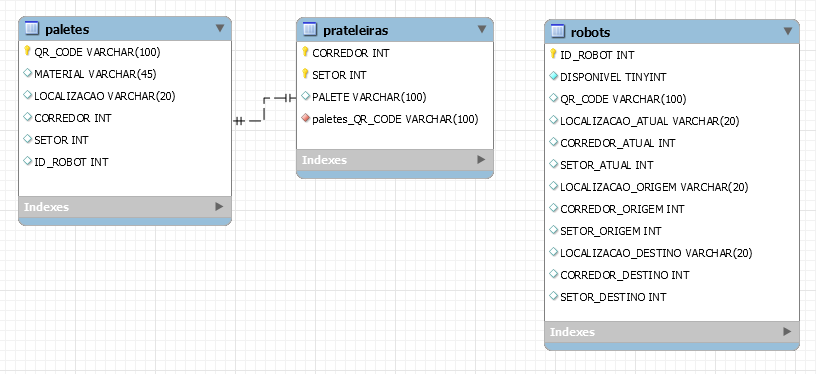
\includegraphics[width=1\textwidth]{images/logicoDSSImage.png}
    \caption{Modelo Lógico}
    \label{fig:my_label3}
\end{figure}

\section{Packages}

O nosso trabalho está dividido em três packages diferentes, sendo eles o bussiness, data e ui. De seguida, procedemos à explicação de cada um deles.

\subsection{Bussiness}

De modo a termos uma melhor organização do nosso trabalho também guardamos as diferentes classes do package Bussiness em diferentes packages sendo eles o comparators, enums, exceptions, localizacao, palete, prateleira e robot. Por fim, temos a classe ArmazemFacade e a interface IArmazemFacade.

\subsubsection{Comparators}

Decidimos criar um comparator de modo a compararmos as distâncias de dois robots e, assim, escolhermos aquele que está mais próximo para a realização da tarefa pendente.

\subsubsection{Enums}

Procedemos à elaboração de dois enums, um deles, o RobotRequest, onde especifica se o request do nosso robot é uma recolha ou uma entrega e o outro, o ZonaArmazem, onde especifica qual a zona do armazém onde se encontra uma determinada palete, ou seja, se numa zona de entrega, numa zona de recolha, numa zona armazenamento ou num robot. Por fim, criamos um Enum vertex onde convertemos a localização num tipo mais simples. 

\subsubsection{Exceptions}

Ao longo da realização do projeto fomo-nos apercebendo de que seria necessário existir algumas exceptions de modo a este ficar mais complexo e mais aproximado da realidade. Deste modo, fizemos quatro exceptions, a EmptyTransportQueueException que trata do caso em que não há paletes para transportar, a InvalidQRCodeException que trata do caso em que o QR Code lido é inválido, a InvalidRequestFromRobot que trata do caso em que o pedido feito é inválido e a InvalidRobotIDException que trata do caso em que o id do robot é inválido.

\subsubsection{Localização}

Para realizarmos a implementação da localização no nosso projeto tivemos de pensar qual seria a melhor abordagem. Assim, o grupo chegou à conclusão que iria criar uma classe abstrata Localizacao que iria ter como atributo uma ZonaArmazem, que é um enum, e depois criar três classes que iriam extender a classe abstrata que seriam as classes Localizacao Armazenamento, que tem como parâmetros dois ints referentes ao setor e ao corredor da palete, Localizacao Robot, que tem como atributo o id do robot que transporta a palete, e Localizacao Transporte.

\subsubsection{Palete}

De modo a implementarmos uma palete no nosso trabalho decidimos que teríamos de criar três classes. Assim surgiram a classe Material que tem como atributo uma string com a designação do produto que a palete contém, a classe QR Code que tem como atributo um inteiro com o código qr da palete e a classe Palete que tem como atributos um QR Code, um Material e uma Localizacao.

\subsubsection{Prateleira}

A classe Prateleira é composta por uma Localizacao Armazenamento e por uma string com o código qr.

\subsubsection{Robot}

Para a realização das tarefas do robot criámos uma classe Entrega que tem como atributos uma String com o código qr e duas Localizacao, sendo elas a origem e o destino da entrega. De seguida, criámos a classe Robot que tem como atributos um inteiro com o seu id, um boolean para saber se este se encontra disponível, uma Localizacao para sabermos a sua localizacao atual e uma Entrega para sabermos a entrega atual do mesmo.

\subsubsection{GrafoArmazem}

Decidimos também criar uma classe GrafoArmazem em que basicamente convertemos o nosso armazém num grafo com recurso à biblioteca jgrapht. De seguida, utilizamos o algoritmo de Dijkstra para perceber qual era o robot mais próximo para recolher uma palete. Foi este o melhor método encontrado pelo nosso grupo para a realização desta tarefa.

\subsubsection{ArmazemFacade}

A classe ArmazemFacade foi feita de modo a implementarmos o nosso sistema. Deste modo, esta classe contém todos os atributos e métodos necessários para a implementação dos use cases dados pelos docentes da unidade curricular.

\subsubsection{IArmazemFacade}

É a interface do nosso sistema.

\subsection{Data}

O package Data contém todas as classes e interfaces referentes a DAO. Estas foram utilizadas de modo a conseguirmos fazer uma conexão entre todas as classes acima descritas programadas em Java com as Bases de Dados que criamos em SQL. Também se neste package o povoamento feito para a Base de Dados do projeto.

\subsubsection{DAOconfig}

Classe que serve para configurar a nossa base de dados.

\subsubsection{PaleteDAO}

Esta classe implementa a interface IPaleteDAO. Tendo em conta os métodos acima referidos, ao criarmos os DAO's para cada um dos Maps/Lists do nosso projeto vimos a necessidade de criar novos métodos. Assim, nesta classe adicionamos os métodos size para saber o número de paletes da base de dados, isEmpty para saber se esta se encontrava vazia, containsKey que verifica se um código qr de uma palete existe na base de dados, containsValue que verifica se uma palete existe na base de dados, get para obtermos uma palete através do seu códgio qr, put para inserir uma palete na base de dados, remove para remover uma palete da base de dados através do seu código qr, putAll para adicionarmos um conjunto de paletes à bd, clear para apagar todas as paletes, métodos para obter diferentes sets e atualizaLocalizacao que, dado um código qr de uma palete, atualiza a localização dessa mesma palete.

\subsubsection{PrateleiraDAO}

A classe implementa a interface IPrateleiraDAO. Esta conta com basicamente os mesmo métodos da classe PaleteDAO, destacando apenas os métodos inserePalete e removePalete que fazem exatamente o que o próprio nome do método indica.

\subsubsection{RobotDAO}

A classe implementa a interface IRobotDAO. Esta classe funciona da mesma forma que as duas classes acima mencionadas aplicando apenas os métodos a uma entidade diferente, neste caso, o Robot. Destacamos apenas o método encontraChegada que é utilizado para alterar os parâmetros do Robot quando este recolhe uma entrega. 

\subsection{User Interface (UI)}

Este package contém as classes que vão tratar das views do nosso projeto.

\subsubsection{Menu}

A classe Menu implementa um menu em modo texto.

\subsubsection{TextUI}

A classe TextUI implementa a interface em modo texto.

\subsection{Conclusão e Análise Crítica Global dos Resultados Obtidos}

Na primeira fase do nosso projeto foi-nos pedida uma análise mais abstrata da aplicação que iríamos desenvolver. A abordagem do grupo inicializou-se pelo desenvolvimento do modelo de Domínio onde estabelecemos quais as principais entidades do nosso projeto bem como as relações que estas estabelecem entre si. Apesar de termos tido alguns contratempos e discutirmos diferentes interpretações do enunciado do projeto encontramos um consenso e pensamos ter conseguido atingir o objetivo proposto. De seguida, e ainda na mesma fase, começamos a desenvolver os diferentes Use Cases que achavamos pertinentes de forma a obtermos uma aplicação com as diversas funcionalidades pretendidas. Nesta fase do projeto, faltaram-nos os Use Cases de iniciar e terminar sessão sendo que de resto pensamos em tudo o que era necessário para o desenvolvimento do projeto. Porém, ao inicializarmos a segunda fase do projeto apercebemo-nos de que em alguns casos tinhamos sido demasiado minuciosos, o que nem sempre era bom para a realização do trabalho.

Com a segunda fase do projeto, adicionamos os Use Cases que nos faltavam e melhoramos também alguns dos que já tinhamos. Nesta fase foi-nos pedido para elaborarmos um diagrama de classes, os diagramas de sequência para cada Use Case, o diagrama de packages e o diagrama de componenentes. A maior dificuldade encontrada pelo grupo foi durante o procedimento de criação dos diagramas de sequência pois já tivemos de pensar nos métodos que iríamos precisar para a implementação da nossa aplicação e em como arranjar a melhor maneira de funcionar tudo em conjunto.

Chegando à terceira fase do projeto, apercebemo-nos de que grande parte do nosso trabalho já estava feito. Toda a modelação e estruturação do projeto já tinha sido feita nas duas fase anteriores. Deste modo, partimos para a implementação da solução final. Pelo caminho deparamo-nos com alguns erros tanto no nosso diagrama de classes como nos nossos diagramas de sequência e voltamos atras para os resolver de forma a obtermos uma aplicação funcional e eficaz e voltamos a trabalhar na implementação.

Concluindo, com este projeto o nosso grupo aprendeu a trabalhar melhor em equipa e em como estruturar e modelar um projeto antes de o começar a implementar. Foi, sem dúvida, um método diferente daquele a que até agora estavamos habituados e todo o trabalho foi bastante desafiante. Desta forma, ficamos a compreender que através de um bom planeamento conseguimos obter um código muito mais conciso e eficaz. Assim sendo, o "percurso" utilizado na realização do nosso projeto foi sempre o mesmo. Começamos por elaborar um determinado Use Case como, por exemplo, "Notificar Recolha de Palete". De seguida, percebendo qual era o ator e o que acontecia procedemos à realização do respetivo diagrama de sequência e, por último, à implementação da solução do Use Case no nosso projeto. Todo este processo ajuda a ter um trabalho mais rigoroso e organizado.

Desta forma, pensamos que, apesar de algumas falhas que aconteceram durante o processo de realização do projeto e que tentamos sempre resolver e melhorar ao longo das três fases, o grupo conseguiu atingir tanto os objetivos impostos por si próprios tanto como pelos docentes da unidade curricular e conceber uma aplicação totalmente funcional e intuitiva.

\end{document}


